%%%%%%%% ICML 2024 EXAMPLE LATEX SUBMISSION FILE %%%%%%%%%%%%%%%%%

\documentclass{article}

% Recommended, but optional, packages for figures and better typesetting:
\usepackage{microtype}
\usepackage{graphicx}
\usepackage{subfigure}
\usepackage{booktabs} % for professional tables

% hyperref makes hyperlinks in the resulting PDF.
% If your build breaks (sometimes temporarily if a hyperlink spans a page)
% please comment out the following usepackage line and replace
% \usepackage{icml2024} with \usepackage[nohyperref]{icml2024} above.
\usepackage{hyperref}


% Attempt to make hyperref and algorithmic work together better:
\newcommand{\theHalgorithm}{\arabic{algorithm}}

% If accepted, instead use the following line for the camera-ready submission:
\usepackage[accepted]{icml2024}

% For theorems and such
\usepackage{amsmath}
\usepackage{amssymb}
\usepackage{mathtools}
\usepackage{amsthm}

% if you use cleveref..
\usepackage[capitalize,noabbrev]{cleveref}

%%%%%%%%%%%%%%%%%%%%%%%%%%%%%%%%
% THEOREMS
%%%%%%%%%%%%%%%%%%%%%%%%%%%%%%%%
\theoremstyle{plain}
\newtheorem{theorem}{Theorem}[section]
\newtheorem{proposition}[theorem]{Proposition}
\newtheorem{lemma}[theorem]{Lemma}
\newtheorem{corollary}[theorem]{Corollary}
\theoremstyle{definition}
\newtheorem{definition}[theorem]{Definition}
\newtheorem{assumption}[theorem]{Assumption}
\theoremstyle{remark}
\newtheorem{remark}[theorem]{Remark}

% Todonotes is useful during development; simply uncomment the next line
%    and comment out the line below the next line to turn off comments
%\usepackage[disable,textsize=tiny]{todonotes}
\usepackage[textsize=tiny]{todonotes}


% The \icmltitle you define below is probably too long as a header.
% Therefore, a short form for the running title is supplied here:
\icmltitlerunning{Submission and Formatting Instructions for ICML 2024}

\begin{document}

\twocolumn[
\icmltitle{Reproducibility Report for VQ-fMRI \cite{chenRethinkingVisualReconstruction2023}}

% It is OKAY to include author information, even for blind
% submissions: the style file will automatically remove it for you
% unless you've provided the [accepted] option to the icml2024
% package.

% List of affiliations: The first argument should be a (short)
% identifier you will use later to specify author affiliations
% Academic affiliations should list Department, University, City, Region, Country
% Industry affiliations should list Company, City, Region, Country

% You can specify symbols, otherwise they are numbered in order.
% Ideally, you should not use this facility. Affiliations will be numbered
% in order of appearance and this is the preferred way.
\icmlsetsymbol{equal}{*}

\begin{icmlauthorlist}
\icmlauthor{Bahman Rouhani}{equal,yyy}
\icmlauthor{Yiqian Liu}{equal,yyy}
\end{icmlauthorlist}

\icmlaffiliation{yyy}{York University, Canada}

\icmlcorrespondingauthor{Bahman Rouhani}{brouhani@yorku.ca}
\icmlcorrespondingauthor{Yiqian Liu}{yql@yorku.ca}

% You may provide any keywords that you
% find helpful for describing your paper; these are used to populate
% the "keywords" metadata in the PDF but will not be shown in the document
\icmlkeywords{fMRI, Vector Quantization, VAE}

\vskip 0.3in
]

% this must go after the closing bracket ] following \twocolumn[ ...

% This command actually creates the footnote in the first column
% listing the affiliations and the copyright notice.
% The command takes one argument, which is text to display at the start of the footnote.
% The \icmlEqualContribution command is standard text for equal contribution.
% Remove it (just {}) if you do not need this facility.

%\printAffiliationsAndNotice{}  % leave blank if no need to mention equal contribution
\printAffiliationsAndNotice{\icmlEqualContribution} % otherwise use the standard text.

\begin{abstract}
This report is for the course project of EECS6322 Winter 2024. An fMRI-to-image model, VQ-fMRI \cite{chenRethinkingVisualReconstruction2023} was selected for this reproducibility challenge. We were unable to fully reproduce the original results but possible reasons are discussed in the report.
\end{abstract}

\section{Paper Summary}
\label{submission}

The selected paper proposed an fMRI-to-image model named VQ-fMRI, which was based on VQ-VAE \cite{oordNeuralDiscreteRepresentation2018}. Vector quantization VAE is a derivation of regular VAE by replacing the continuous latent space with a discrete one. This discrete latent space was represented by a codebook containing a limited number of prototype vectors. An encoded image now consists of these prototype vectors at a lower spatial resolution.

The proposed VQ-fMRI model first needs a trained VQ-VAE including its codebook, independent of fMRI data. Then, an fMRI encoder is guided by the codebook to learn to encode fMRI recordings to the discrete prototype vectors. After a series of learned de-noising and content completion processes for the encoded fMRI, it is decoded by the VQ-VAE decoder to reconstruct the image shown to the fMRI subject. Therefore, the reconstructed image uses information from both visual stimulus (fMRI) and past experience (codebook), which is one of the motivations of the paper.


\subsection{Paper Contributions}
As stated by the authors and observed by us, the main contributions of the paper are:
\begin{itemize}
\item The Vector-Quantization fMRI decoding framework that uses both current signals and past knowledge to reconstruct images.
\item The learned denoising and inpainting processes for encoded fMRI data, where the denoiser predicts at which spatial locations are the prototypes valid, and the inpainter completes the latent visual cue by replacing the invalid prototypes.
\item The downsampling and super-resolution component on the fMRI side that reduces the encoder's bias towards high-frequency features.
\item Better results comparing to previous methods.
\end{itemize}


\section{Reproduction Attempt}

We planned to reproduce the main reconstruction results including their evaluation. There were four components that needed implementation and training:
\begin{itemize}
\item Phase I: VQ-VAE
\item Phase II: fMRI encoder
\item Phase III: denoiser and inpainter
\item Phase IV: super-resolution model
\end{itemize} 

After implementation with PyTorch, we first trained VQ-VAE on ImageNet as all remaining components are dependent on it. The fMRI encoder was then trained using the quantizer of VQ-VAE and the GOD dataset \citep{horikawa2016}, which contains fMRI recordings from five subjects and corresponding images. The denoiser, inpainter, and super-res model were trained last. Lab desktops and own laptops were the main computation resources we leveraged in this project.

\subsection{Our Results}

\begin{figure}[t]
\begin{center}
\centerline{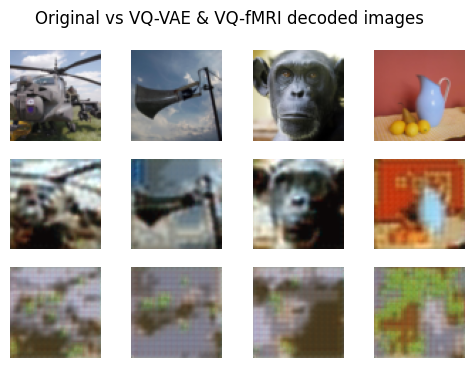
\includegraphics[width=\columnwidth]{decoded-imgs}}
\caption{Our reproduction results. First, second and third row shows the stimulus, the VQ-VAE decoded and the VQ-fMRI decoded images, respectively. Images were selected randomly.}
\label{decoded-imgs}
\end{center}
\vskip -0.2in
\end{figure}

\begin{figure}[!t]
\begin{center}
\centerline{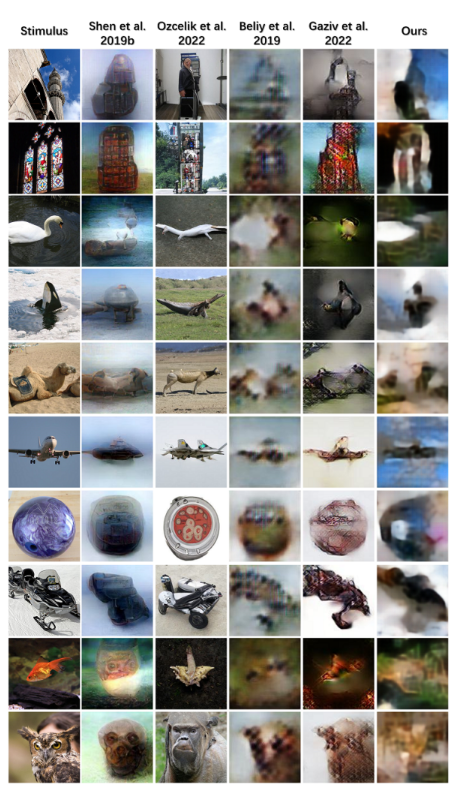
\includegraphics[width=\columnwidth]{orig-figure}}
\caption{Results from original paper, Fig 5 \citep{chenRethinkingVisualReconstruction2023}. First column shows the stimulus images, and last column shows their VQ-fMRI decoded images.}
\label{orig-figure}
\end{center}
\vskip -0.2in
\end{figure}


\textbf{Qualitative results. TODO}
As shown in \cref{decoded-imgs}, ...
Comparing the last row of \cref{decoded-imgs} to the last column of original results in \cref{orig-figure}, they clearly had better color restoration and the outlines seemed smoother with more details.


As a side note, our trained VQ-VAE did not produce as good results (\cref{decoded-imgs}, 2nd row) as in \cite{oordNeuralDiscreteRepresentation2018}.


\textbf{Quantitative results. TODO} \cref{metric-table} shows the comparison of evaluation metrics between the original results and our reproduction. ...

\medskip

Other than above evaluation results, we could confirm that shape info were learned before color and texture info over the course of training, as claimed in the paper.

\subsection{Possible Reasons for Discrepancies TODO}
although reasonable amount of details are provided in the paper ....



TO REMOVE

The text of the paper should be formatted in two columns, with an
overall width of 6.75~inches, height of 9.0~inches, and 0.25~inches
between the columns. The left margin should be 0.75~inches and the top
margin 1.0~inch (2.54~cm). The right and bottom margins will depend on
whether you print on US letter or A4 paper, but all final versions
must be produced for US letter size.
Do not write anything on the margins.

The paper body should be set in 10~point type with a vertical spacing
of 11~points. Please use Times typeface throughout the text.


%\subsection{Figures}
%You may float figures to the top or
%bottom of a column, and you may set wide figures across both columns
%(use the environment \texttt{figure*} in \LaTeX). Always place
%two-column figures at the top or bottom of the page.

\subsection{Tables}

You may also want to include tables that summarize material. Like
figures, these should be centered, legible, and numbered consecutively.
However, place the title \emph{above} the table with at least
0.1~inches of space before the title and the same after it, as in
\cref{sample-table}. The table title should be set in 9~point
type and centered unless it runs two or more lines, in which case it
should be flush left.

% Note use of \abovespace and \belowspace to get reasonable spacing
% above and below tabular lines.

\begin{table}[t]
\caption{Comparison of quantitative evaluation metrics.}
\label{metric-table}
\vskip 0.15in
\begin{center}
\begin{small}
\begin{sc}
\begin{tabular}{lrrc}
\toprule
Metric & Original & Ours & Reproduced? \\
\midrule
SSIM    & 0.492 & TODO & $\times$ \\
PSNR    & 13.4 &  TODO & $\times$ \\
PCC     & 0.551 & TODO & $\times$ \\
\bottomrule
\end{tabular}
\end{sc}
\end{small}
\end{center}
\vskip -0.1in
\end{table}

Tables contain textual material, whereas figures contain graphical material.
Specify the contents of each row and column in the table's topmost
row. Again, you may float tables to a column's top or bottom, and set
wide tables across both columns. Place two-column tables at the
top or bottom of the page.


\section{Contribution of Team Members}
We believed the workload split between two of us was even. Before project proposal, we independently looked for appropriate papers, and each short-listed about 3 of them. We agreed on this VQ-fMRI paper that interested both of us.

The proposal document was mostly written by Bahman; this report was mainly prepared by Yiqian. Bahman recorded the presentation video.

In terms of implementation, we tried to followed the planned work split in the proposal. Bahman coded for vector quantizer of VQ-VAE, and UNet, which was used in multiple components of the final model, including the inpainter, denoiser, and super-res model. Bahman also wrote some data loaders and training code. Yiqian designed the high-level structure and the interfaces. Yiqian also coded up the image encoder \& decoder of VQ-VAE, fMRI encoder, some training, and evaluation. Occasionally, we corrected each other's code.

During model training, Yiqian was responsible for VQ-VAE (Phase I) and fMRI encoder (Phase II), whereas Bahman took over denoiser \& inpainter (Phase III) and super-res model (Phase IV).


\section*{Software and Data TODO}

If a paper is accepted, we strongly encourage the publication of software and data with the
camera-ready version of the paper whenever appropriate. This can be
done by including a URL in the camera-ready copy. However, \textbf{do not}
include URLs that reveal your institution or identity in your
submission for review. Instead, provide an anonymous URL or upload
the material as ``Supplementary Material'' into the OpenReview reviewing
system. Note that reviewers are not required to look at this material
when writing their review.

% Acknowledgements should only appear in the accepted version.
\section*{Acknowledgements}

\textbf{Do not} include acknowledgements in the initial version of
the paper submitted for blind review.

If a paper is accepted, the final camera-ready version can (and
probably should) include acknowledgements.


% In the unusual situation where you want a paper to appear in the
% references without citing it in the main text, use \nocite
%\nocite{langley00}

\bibliography{report}
\bibliographystyle{icml2024}

\end{document}


% This document was modified from the file originally made available by
% Pat Langley and Andrea Danyluk for ICML-2K. This version was created
% by Iain Murray in 2018, and modified by Alexandre Bouchard in
% 2019 and 2021 and by Csaba Szepesvari, Gang Niu and Sivan Sabato in 2022.
% Modified again in 2023 and 2024 by Sivan Sabato and Jonathan Scarlett.
% Previous contributors include Dan Roy, Lise Getoor and Tobias
% Scheffer, which was slightly modified from the 2010 version by
% Thorsten Joachims & Johannes Fuernkranz, slightly modified from the
% 2009 version by Kiri Wagstaff and Sam Roweis's 2008 version, which is
% slightly modified from Prasad Tadepalli's 2007 version which is a
% lightly changed version of the previous year's version by Andrew
% Moore, which was in turn edited from those of Kristian Kersting and
% Codrina Lauth. Alex Smola contributed to the algorithmic style files.
